\chapter{Flat Scan Sampling}

	Background for the Flat Scan Sampling (FSS) method and a general description are presented along with the writers C++ implementations and an analysis of the single core and parallel performance.

\section{Background}

	The author of FSS, João Amaral, had previously, in 2014, proposed a new method to estimate the JDoS, Random Path Sampling (RPS).  The RPS was implemented in high performance languages and extensively studied by Nuno Fortunato.  (citar)
	
\begin{figure}[h]
	\centering
	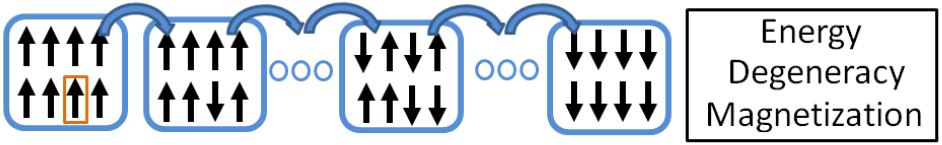
\includegraphics[scale=0.35]{rps_diagram.png}
	\caption{Scheme of how the Random Path Sampling method works.}
	\label{rps_dia}
\end{figure}
	
	The RPS method departs from the premise that by starting on an extreme magnetization point in the phase space, generally all spins up $(M)$, and successively flipping one spin down at each step of the random walk, we arrive at the other end of the phase space $(-M)$. Process illustrated in Figure \ref{rps_dia}. Performing $R$ sweeps of the phase space generate a histogram that is flat in magnetization and we can obtain the JDoS by 
\begin{align}
	H(E, M)/R &= P(E, M), \\
	\Omega(M) \times P(E, M) &= g(E, M).
\end{align}
$\Omega(M)$ is defined in Equation \ref{norm_fact}.

	The idea for FSS departs from the basic mechanism of RPS, in the sense that it is a method that estimates the JDoS by a sequential sweep of the phase space magnetization by magnetization. However the way of that both methods sample the phase space is completely different. The FSS takes a similar approach to the WL method, in the sense that a random walk with probability proportional to the inverse of the DoS is performed, a flat energy random walk.
	
	\pagebreak

\section{Algorithm}

	The Flat Scan Sampling method stems from the observation that if  the DoS at a certain magnetization $M_q$ is known, by performing a random walk the energy space $(E, M_q)$, with a probability proportional to the inverse of the DoS $\frac{1}{g(E)}$, called a flat energy random walk, and by sampling a set number of statistically diverse configurations for each energy value the DoS at the next magnetization $M_{q+1}$ can be estimated. 
This is possible because at each step of the random walk we perform a scan, i.e., in a sequential manner, we flip and unflip each spin in our configuration obtaining information about the DoS at the next magnetization, $g(E, M_{q+1})$. 
The value of $g(E_j, M_{q+1})$ is then computed through the value of $g(E_i, M_q)$ by the following equation
\begin{equation}\label{eq:FSS_JDoS}
	g(E_j, M_{q+1}) = g(E_i, M_q) \times \text{fraction of configurations}.
\end{equation}

\begin{figure}[h]
	\centering
	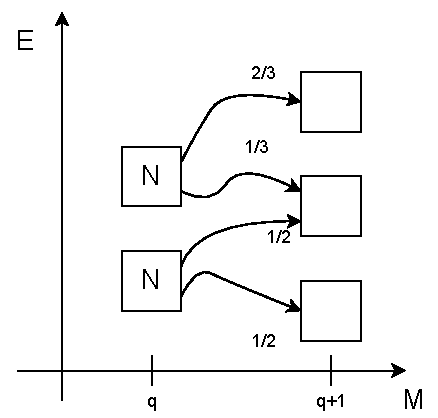
\includegraphics[scale=0.55]{fss_diagram.pdf}
	\caption{Scheme of how the Flat Scan Sampling works.}
	\label{fss_dia}
\end{figure}

Shown in Figure \ref{fss_dia}, the fraction of configurations corresponds to the fraction of the scanned configurations in the random walk that contributed to the estimation of the DoS at the next magnetization. This way, the JDoS is computed sequentially by starting at a known DoS in the phase space, such as all of the spins up $(M)$, and sweeping the whole phase space magnetization by magnetization until we arrive at the configuration where all of the spins are down $(-M)$.

The principal parameter of the method is the maximum number of samples for each point in the energy space, known as REP. In later section new parameters will be introduced to try to make the estimation more accurate while sacrificing some performance.  There will be also an extensive study of how this parameters affects the precision of the JDoS and wall time.

The algorithm can be written in the following steps:
\begin{enumerate}
\item Choose a magnetization value where $g(E, M_q)$ is known, usually magnetization where the spins all up/down;
\item Generate a certain configuration in that magnetization and compute its energy, $E_i$;                                                                                                                                       
\item Choose a spin to flip down and another one to flip up and compute the energy of the new configuration, $E_j$;
\item Accept the new configuration with a probability $\min(1, g(E_i)/g(E_j))$;
\item Sequentially flip each spin in the configuration, taking the system from the state $(E_i, M_q)$ to $(E_j, M_{q+1})$ and accumulate a histogram $H(E_i, E_j)$ and unflip the spins;
\item If the all of the number of sampled states per $(E,M_{q})$ pair is equal to REP, stop the simulation and compute the DoS at $q+1$ by using Equation \ref{eq:FSS_JDoS}. Where the fraction of configurations is now equal to $H(E_i, E_j)/\sum_j(H(E_i,E_j))$.
\end{enumerate}

\section{CPU Implementation}

	For single core and message passing interface (MPI) implementations, C++ was the preferred because of its speed and optimization over python or MatLab, and modularity, over C. The random number generator (RNG) used was the xoshrio256**.

	Before the description of the implementation let us define the function that handles the scan. This should be performed each step of the simulation. The scan is defined as flipping each spin in the configuration, measuring the new energy and registering the change in state $E_i \rightarrow E_j$ in the histogram. Thus, this operation can be implemented with a for cycle running from $0$ to $N$, the number of spins.
\begin{algorithm}
	\begin{algorithmic}[1]
	\Function{\texttt{scan}}{\texttt{configuration}}	
		\For {\texttt{idx = 0,1,..., N-1}}
			\State flip the spin \texttt{idx} spin down
			\State compute the new energy \texttt{Ej}
			\State \texttt{H(Ei, Ej)++}
			\State flip the spin \texttt{idx} spin up
		\EndFor
	\EndFunction
	\end{algorithmic} 
\end{algorithm} 

	The actual implementation follows the base-line algorithm described in the last section. By knowing that the JDoS is symmetric, to save computing time, we can estimate only half of the JDoS and after the simulation mirror it. Here \texttt{qmax} is the index of the last magnetization in our computation. The variable \texttt{hist(E)} is used to count how many configurations were sampled in each point of the energy space. We only stop when every point has sampled REP microstates. In pseudo-code it can be written as follows 
	
\begin{algorithm}
	\begin{algorithmic}[1]
		\For {\texttt{q=0,1,...,qmax}}
		 	\State set \texttt{hist(E) = 0} and \texttt{H(Ei,Ej)=0}
		 	\State generate random configuration with \texttt{M=Mq} and compute its energy \texttt{Ei}
		 	\State \texttt{scan(configuration)}
		 	\State \texttt{hist(Ei)++}
		 	\While {\texttt{min(hist(E) < REP)}}
		 		\State flip one random spin down
		 		\State flip one random spin up
		 		\State compute the energy of the new configuration \texttt{Ej}
		 		\State set \texttt{ratio = min(g(Ei)/g(Ej))}
		 		\If {\texttt{rand() < ratio}}
					\State accept new configuration
				\Else
					\State reject new configuration
		 		\EndIf
		 		\If {\texttt{hist(Ei) < REP}}
		 			\State \texttt{hist(Ei)++}
			 		\State \texttt{scan(configuration)}
		 		\EndIf
		 	\EndWhile
		 	\State set \texttt{g(E,Mq+1) = g(E,Mq) * H(Ei, Ej) / sum(H(:,Ej))} 
		 \EndFor
	\end{algorithmic} 
\end{algorithm}

	This implementation has the same problem as the original WL method. We sample successive configurations, thus reducing statistical accuracy and increasing correlation between scans. This way, a new parameter that reduces correlation between scanned configurations is proposed. It is called skip and acts the same way as the parameter $S$ in the WL. We only sample configurations that are distanced by skip steps in the random walk. Only line 17 is modified by the addition of "and \texttt{k \% skip = 0}". Usually this value is set equal to the number of spins in the system, $N$.
	
\section{Validation and Convergence}

\begin{figure}[h]
	\centering
	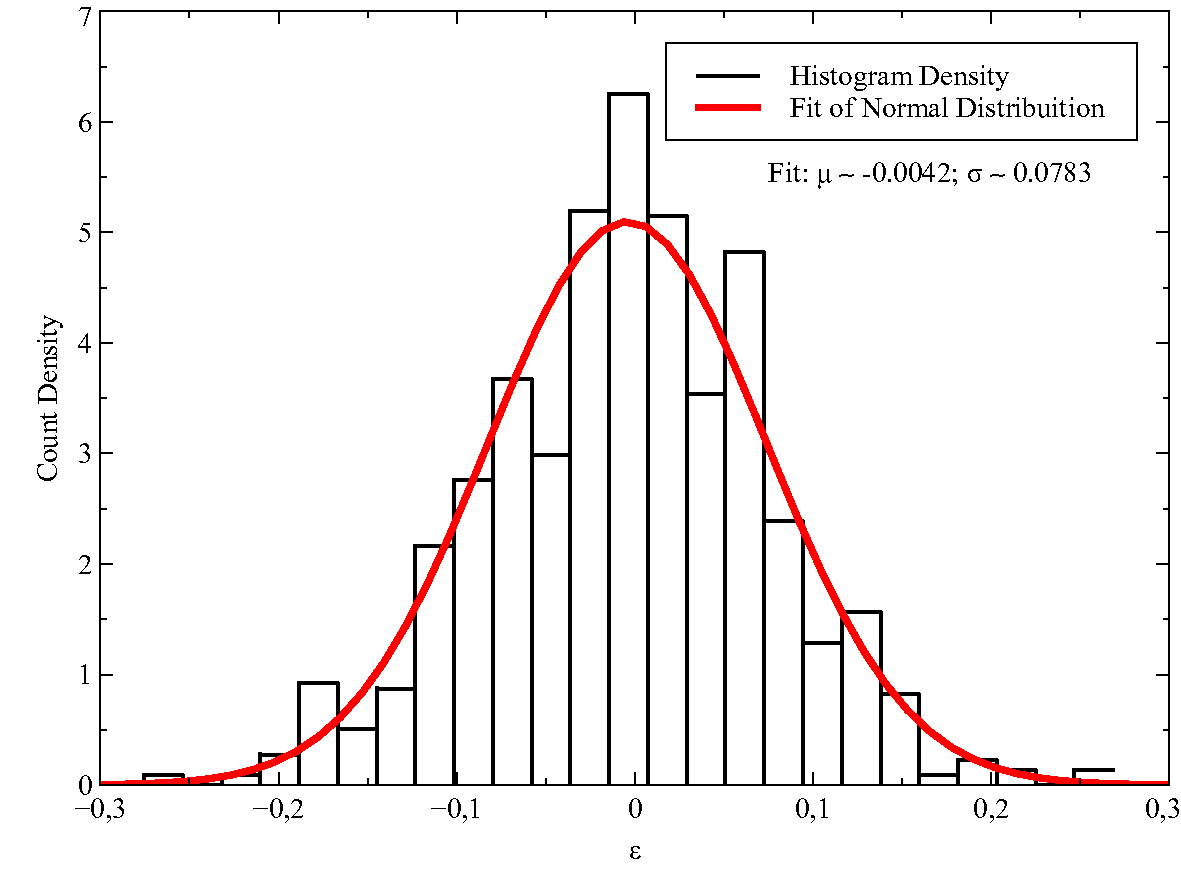
\includegraphics[scale=0.5]{convergence_validation/validation_convergence_01.pdf}
	\caption{Scheme of how the Flat Scan Sampling works.}
\end{figure}

\begin{figure}[h]
	\centering
	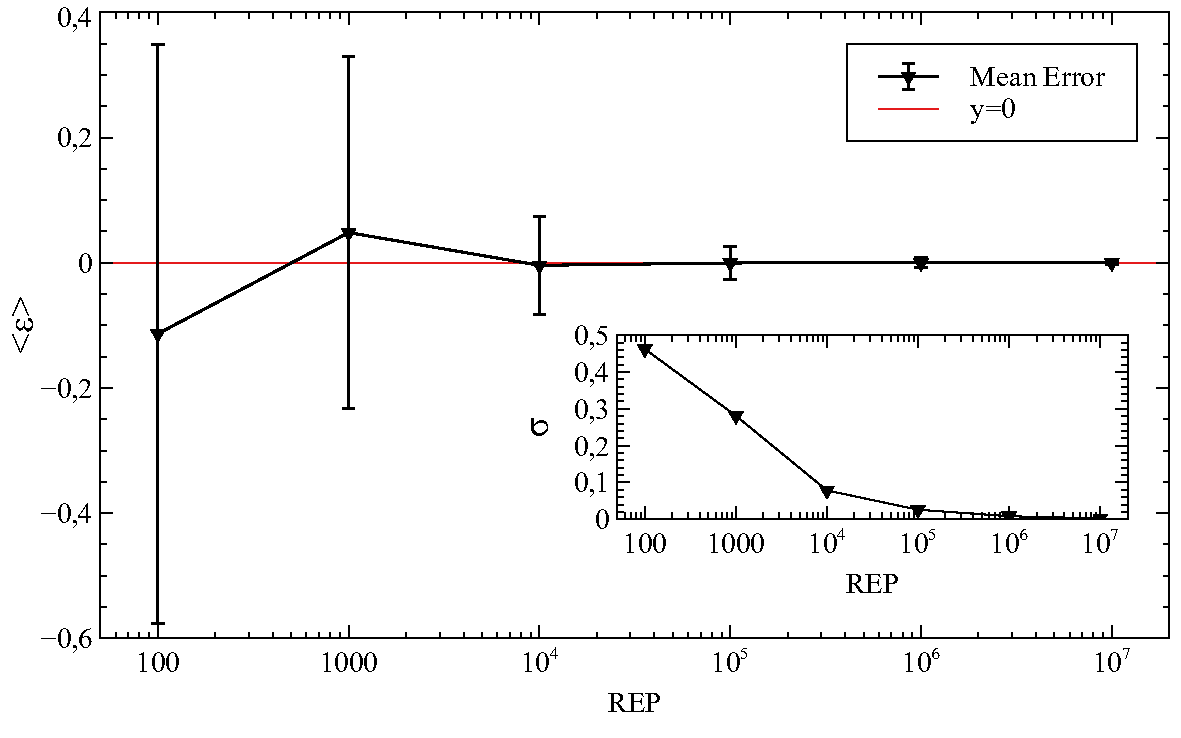
\includegraphics[scale=0.5]{convergence_validation/validation_convergence_02.pdf}
	\caption{Scheme of how the Flat Scan Sampling works.}
\end{figure}

\begin{figure}[h]
	\centering
	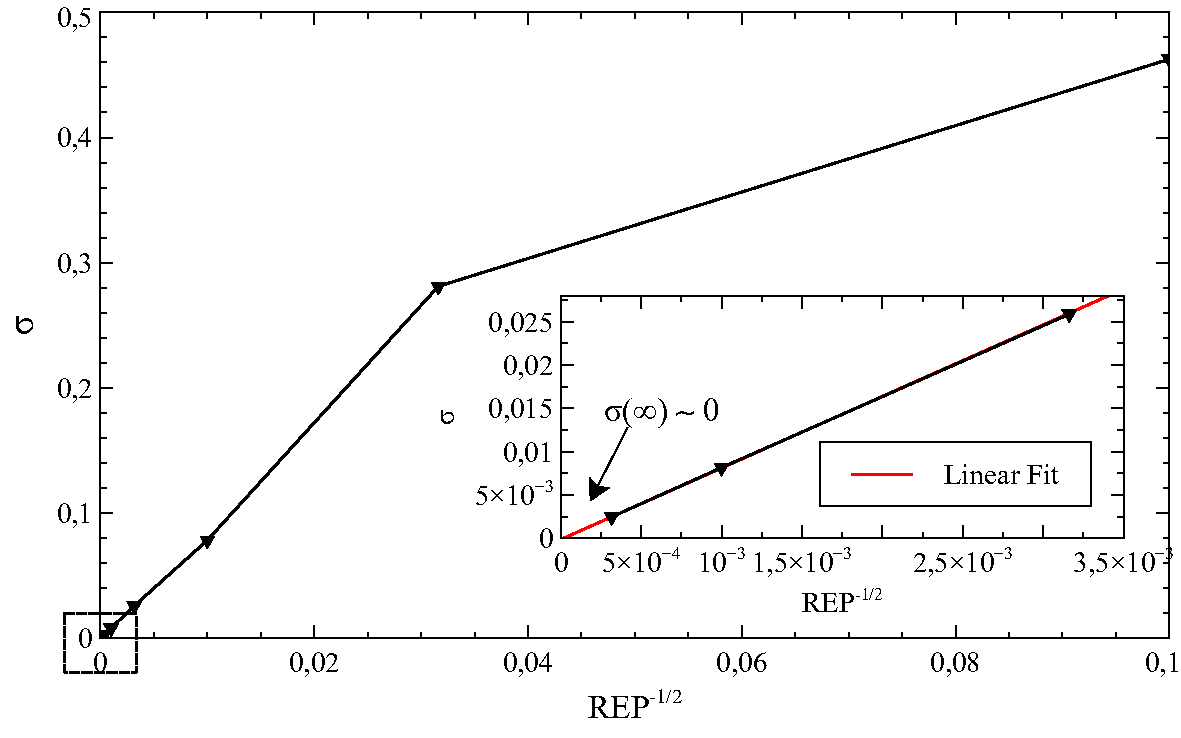
\includegraphics[scale=0.5]{convergence_validation/validation_convergence_03.pdf}
	\caption{Scheme of how the Flat Scan Sampling works.}
\end{figure}

\begin{figure}[h]
	\centering
	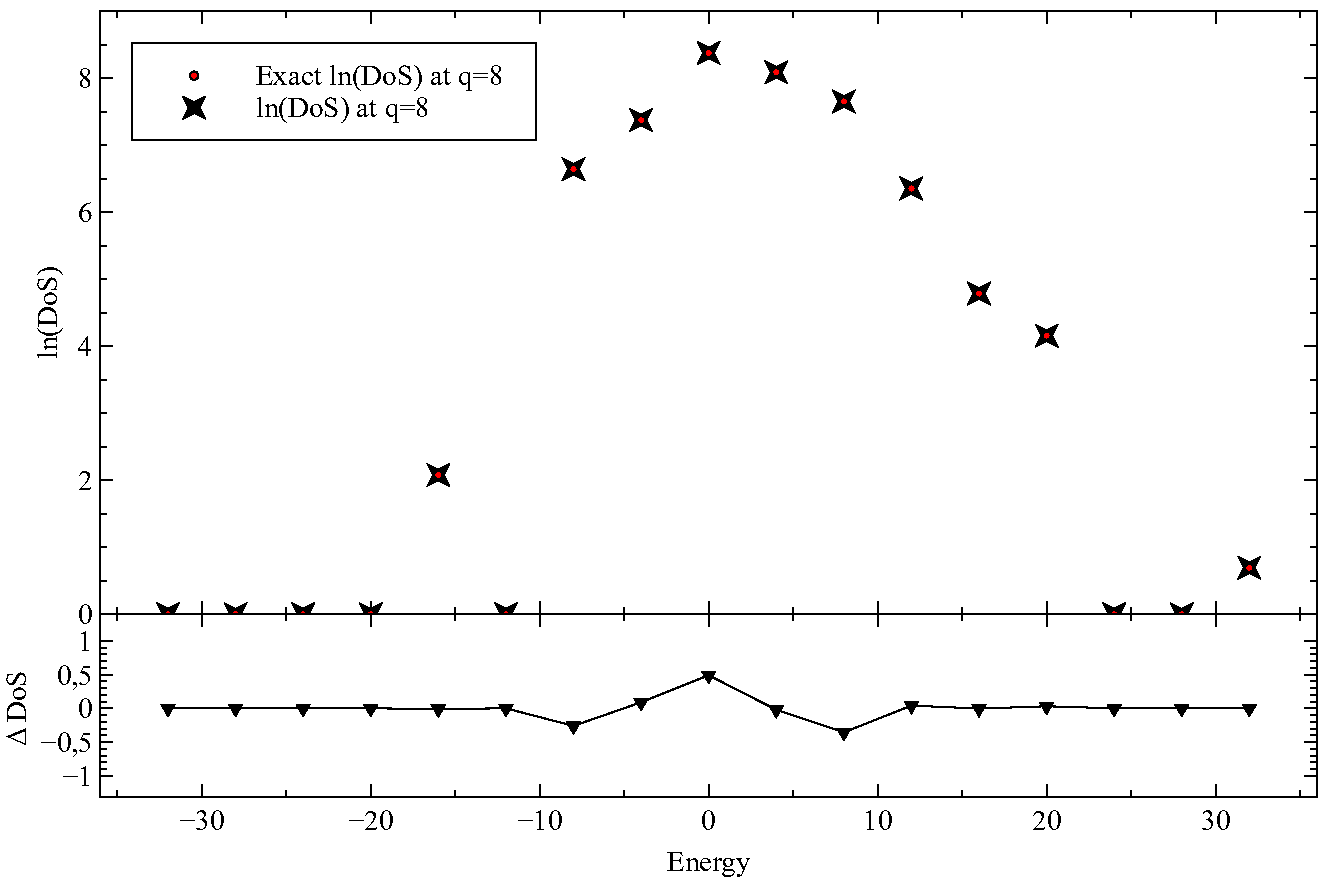
\includegraphics[scale=0.5]{convergence_validation/validation_convergence_04.pdf}
	\caption{Scheme of how the Flat Scan Sampling works.}
\end{figure}

\begin{figure}[h]
	\centering
	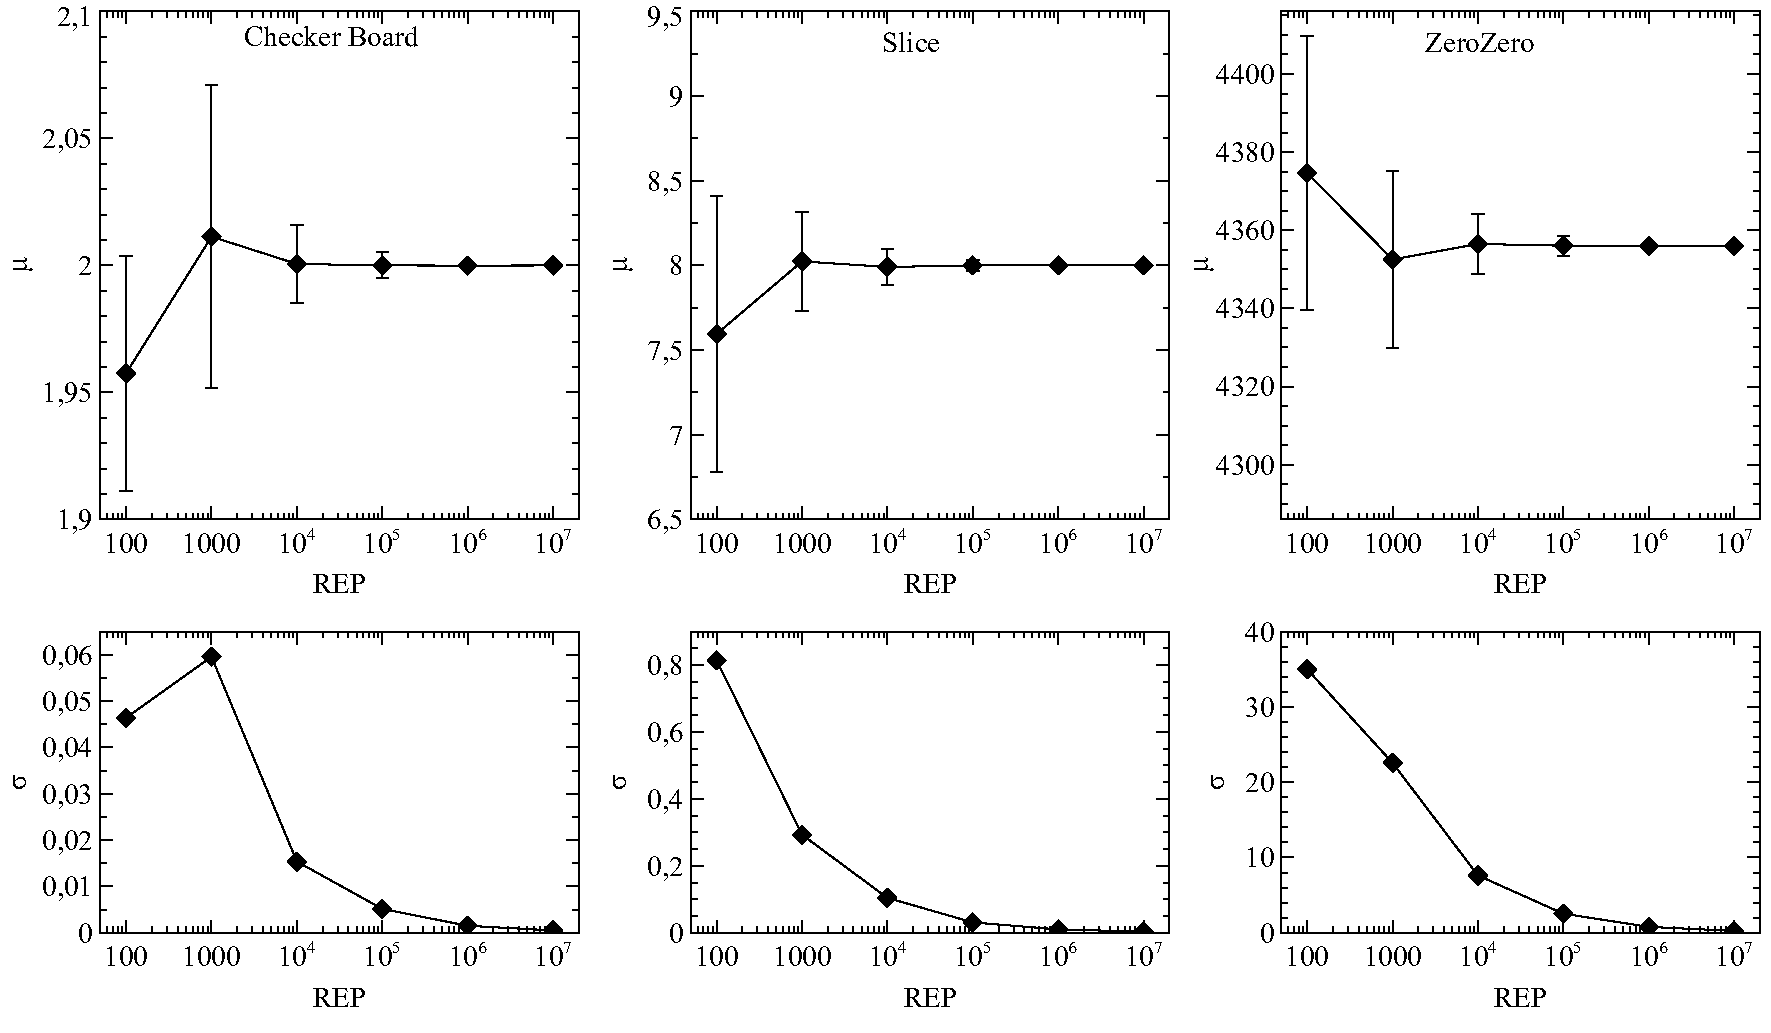
\includegraphics[scale=0.5]{convergence_validation/validation_convergence_05.pdf}
	\caption{Scheme of how the Flat Scan Sampling works.}
\end{figure}

\section{Comparison with Wang-Landau}
























